\documentclass[conference,12pt]{IEEEtran}
\usepackage{pdflscape}
\usepackage{longtable}
\usepackage[bitheight=6ex]{bytefield}
\usepackage{todonotes}
\usepackage{hyperref}
\usepackage{tabularx}
\usepackage{graphicx, subfigure, amsmath} 
\usepackage{pdfpages}
\usepackage[backend=biber,style=ieee]{biblatex}
%\usepackage[section]{placeins}
\addbibresource{References.bib}
\interdisplaylinepenalty=2500

% correct bad hyphenation here
\hyphenation{}


\begin{document}
%
% paper title
\title{Automotive Communications \\ \large{Better Than Best Effort}}

\author{
\IEEEauthorblockN{Jeremy Wright}
\IEEEauthorblockA{Arizona State University\\jlwrigh1@asu.edu}
}
\maketitle
\begin{abstract}
Vehicle's are quickly becoming distributed computing platforms on wheels, and
the integration of these system is essential for both the safety and comfort of
the passengers. Over the last few decades there has been increasing integration
of these systems to perform highly advanced functions, but never losing their
core safety and reliability. This survey will look at the 4 most
popular automotive networks in vehicles, how they differ from the Ethernet based
protocols we are used to in the Internet domain, and how the physical layers and
software layers interact to make a truly safe system. 
\end{abstract}

\begin{IEEEkeywords}
CAN, LIN, MOST, FlexRay, safety, reliability
\end{IEEEkeywords}

\section{Introduction}

Something flashes across the road. Instinctively you slam on the brakes. ABS
kicks in to preserve tire contact with the road. Your body begins to fly
forward, your head towards the steering wheel. Inertial sensors begin to deploy
the air-bag. The fuel pump is shut down to reduce the
risk of fire. Electronic Stability control adjusts suspensions dampers to keep the vehicle
 in a safe driving position. The vehicle signals emergency responders
of a crash event with the current GPS location. The air bag catches you.
The crash is over. You are safe. 

This is the environment of automotive networks.
The hard real-time communication channels where failure means people die.
Internet protocols security is always at the forefront. How confidentiality,
integrity and availability are addressed in is a commonly discussed topic.
Automotive protocols however choose to optimize just two of these aspects, Availability, and Integrity.
Messages must arrive intact, and before the deadline with bounded latency.

CAN was one of the earliest automotive protocols.  Introduced by Bosch in 1983
\autocite{std_can} CAN increased vehicle safety, reduced vehicle weight, and
improved overall comfort of the system \autocite{navet_trends_2005}. Prior to
this software
assisted vehicle functions were connected by point-to-point wiring.  Each
function including it's own wiring harness, and it's own priority protocols.
Not only did this make diagnosing problems difficult, but also resulted in a great deal of
unnecessary cost. As of 2009, Mercedes vehicles are using up to 70 ECUs
\autocite{guo_integrated_2009}. Without a safe multi-access network, such
network would not be possible.  Pointing to a picture of a car, Bjarne
Stroustrup, the inventor of C++, stated, ``...that isn't a car, it is
a distributed computing platform, on wheels...''
\autocite{going_native_keynote_bjarne}.  Additionally, automotive protocols also allow ECUs to work
cooperatively merging sensor data from multiple end points to achieve advanced
vehicle functions. Today, the X-by-wire systems are the epitome of this capable
of detecting road obstructions and even stopping the vehicle if necessary.  

Conversely, Internet protocol is fault
tolerant and employs a concept called best effort routing, where packets are
routed to a destination in the most likely path for success.  Packets have
a time to live, and if they don't reach the destination in time, drop off the
network \autocite{_best-effort_2014}. For a moment, consider a ``best effort'' approach in a vehicle. 
The music
player is shipping data over the vehicle network. The air bag deploy message
cannot get any bandwidth. The airbag would not deploy, and someone could get
very hurt. Instead of best effort, automotive
protocols take a different approach focused on safety, reliability, and
guaranteed delivery. This focus usually is a trade-off for performance.
Automotive networks will not send gigabits per second, but the data you need to
seed will be sent reliability since, when the air bag needs to deploy, being late is useless.

\section{Segregating the Vehicle Network}
The number of ECUs in our vehicles are growing. Each ECU fits into different
services, providing different levels of service. Quality of service is not
common across all network types. 
One level of abstraction above the ECU are the system categories: power-train,
comfort, chassis, and infotainment.  Power-train systems involve engine and transmission
data, and have the very tight timing, and jitter specification since these
systems are responsible for function such as variable valve timing, spark
advance/delay and other critical engine functions. Comfort is the other end of
the spectrum, and provides the environment controls such as AC, heating, and
radio.  Increasingly these comfort systems have grown to include cellular phone
integration, and even Hotspot functionality. This network category requires
higher bandwidth, and higher speed but with a lower emphasis on safety, and
reliability. Late message may disrupt the music, but it will not likely result
in harm.  Chassis systems are responsible for maintaining control of suspension,
steering and braking. These are a high reliability network type.
\autocite{navet_trends_2005}.

This survey will step through three automotive protocols commonly used in
vehicles today: CAN \autocite{std_can}, LIN \autocite{std_lin} and FlexRay
\autocite{std_flexray}.  Each protocol has a defined set of quality
specifications. Each deals with errors, and reliability in a unique way.
Buildign up, we will look at how networks may be composed of these services.  
Vehicle network design takes an approach more similar
to a VoIP network than how one would design a network for email, and
Internet browsing.  In these types of networks latency and jitter are key functions that
translate to real physical requirements. Automotive protocols use customized
physical layers to provide reliability services. Beyond this, the application
layers can extend the reliability somewhat using different messaging schemes.
Today, there are two primary methods Time-Triggered messages, and
Event-Triggered Messages. 

Vehicle functions are segregated into discrete Electronic Control Units (ECUs)
distributed around the vehicle. These ECUs provide raw sensor data, engine
statistics, trouble code information, and even dynamic suspension information,
all in real-time. Before the advent of CAN, these systems were
completely segregated, and often implemented by different vendors e.g. the door
lock system would be physically separated from the truck latch.  Segregated
there was no issue of contention since the system fully owned the communication
channels it needed. However this also resulted in a great deal of redundancy,
cost, and weight.  Furthermore, many functions can have enhanced accuracy or
precision by combining several different data sources in a scheme called sensor
fusion.  CAN was introduced to address these issues.  CAN allowed ECUs to be
linked together with a single twisted pair of copper wires, and included a novel
priority scheme for routing higher priority messages ahead of lower priority
ones.

So how is reliability defined? Within vehicles, reliability maps to the
security concept of availability. The message bus must be available when a high
priority message is to be sent, and the latency must be absolutely bounded.
Furthermore vehicles are electrically very harsh environments. Temperatures can
be extreme, sensors, and system are exposed to weather. Because of this the
physical layers must continue to function in the presence of high electric
fields or magnetic fields or poor EMI environments.  Ethernet for example doesn't meet
this requirement. Within HVAC, one must be carefully to lay Ethernet lines around
fluorescent tube lighting. The magnetic fields generated by the
arching gas can degrade performance at higher speeds
\autocite{center_interesting_ethernet}. In a vehicle this
variably of network quality is unacceptable. 


\section{Reliable Networks}
Reliability is an ECU knowing that
a message sent was received by its intended receiver, and still meeting it's
deadline. Vehicle buses
must allow messages to arrive in a deterministic amount of time. Since messages
could contain life critical instructions such as deploy air bags, highest
priority message must get through. 

This is also related to safety, at the
protocol level, messages must get though. At the signal level vehicles are
electrically very noisy \autocite{paruchuri_inter-vehicular_2011}. Noise can
induce eddy currents or other anomalous bits
in the digital networks. The physical layer must protect against these to
achieve safe operation.  CAN, LIN, and FlexRay all take a different approach to
this issue. LIN for instance pushes error detection up to the application layer,
while FlexRay, and CAN address it with CRCs in the physical layer. Lastly, we will look at time triggered,
verses event triggered message schemes an how each system fits into the overall
safety case. 

Besides reliability networks provide different levels of performance separated by
their class.
\begin{table}[!t]
\renewcommand{\arraystretch}{1.3}
\caption{Network Classes by speed}
\label{tbl:network_classes}
\centering
\begin{tabular}{c c c}
\hline
\bfseries Network Class & \bfseries Speed & \bfseries Typical Use \\ \hline
\hline
A & $< 10$ Kbps  & Body domain \\
B & $< 125$ Kbps & Sensor Sharing \\
C & $< 1$ Mbps   & Power-train and Chassis Domain \\
D & $> 1$ Mbps    & Media and infotainment \\
\hline
\end{tabular}
\end{table}

\subsection{CAN} 
CAN is a Class C, half-duplex network. CAN provides priority based messaging by
implementing an OR function into the physical layer itself. CAN consists of
a shielded - twisted differential pair of copper wires.  The
transceiver sends uses an open collector allowing the logical bus value to float
high to 1. This makes 0 the dominate bit.  When a node wishes to send a message
on the bus, it begins pulling the line down signaling the betting of a frame,
and the id of the message. Simultaneously, the transceiver measures the line to
verify the signal it tried to put on the line, was transfered to the receivers.
In this way the sender immediately knows every bit was successfully sent or not.
Essentially every ECU can begin sending a message at the same time, the message
with the most ones wins, and other senders will back off. This process is call
arbitration, and implements priority at the physical level. Message identifiers
are designed with a balanced number of ones to describe the desired priority
relationships. J1939 is a standard set of CAN identifiers designed for just
purpose \autocite{sae_j1939}.

Besides priority at the physical level, CAN defines this priority scheme should
exist through the transceiver up through the software stack.  The CAN standard
defines that transceivers must have 3 hardware buffers which employ the same
voting scheme. At a high level, when one wishes to send data on the network you
write you messages to 1 of the three hardware buffers in a round-robin fashion.
The hardware then sends the highest priority message as soon as the bus is
available i.e. either the bus is idle, or the current message is the highest
priority and wins arbitration. One level above this, the software stacks should
be implemented as priority queues removing the highest priority messages first
\autocite{std_can}.  In this way, highest priority messages of the system as
a whole are always sent first.  Individual ECUs also schedule their own highest
priority message to be sent first. The physical bus' priority scheme assures that
the highest priority messages are sent on the bus.  

Secondly, CAN deals with the issue of CAN transceivers who are stuck sending high
priority message and flooding the bus with superfluous data. CAN transceivers
include a hardware watchdog looking for error frames. Error frames are always
highest priority and can send ECU's to a buss off mode where they cannot talk at
all giving control back to good citizens of the bus. Implementing this function
contributes to the higher cost of CAN as opposed to buses like LIN. All can
transceivers must be licensed by Bosch to verify they meet the specification.
This license cost is carried by the chip manufactures, which in turn raises the
cost of the devices to implementors. 

To achieve data integrity, each can frame is packed with a 32-bit CRC. 

\begin{figure}
  \centering
  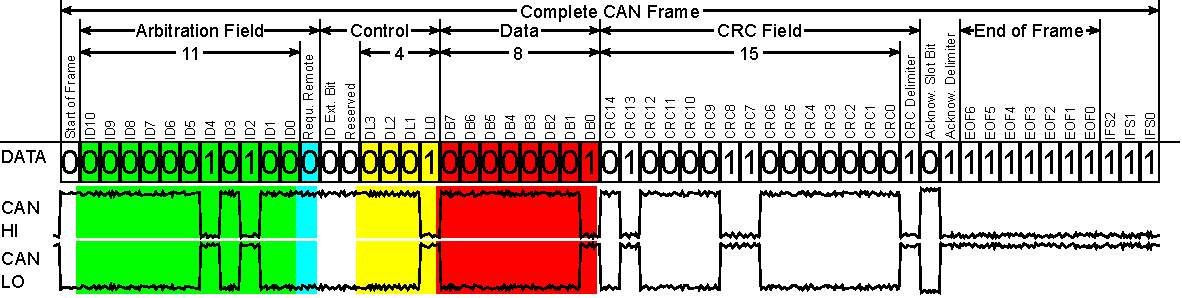
\includegraphics[width=0.4\textwidth]{can_frame.pdf}
  \caption{CAN Frame without bit stuffing}
  \label{fig:can_frame}
\end{figure}

Can was the first industrial protocol for vehicles, and CAN is used for nearly
all systems of a vehicle, except for the comfort system which require higher
bandwidth than CAN provides.

\subsection{LIN}
LIN is a class A, half duplex, master-slave network \autocite{std_lin}. It provides a low
cost network capable of interfacing up to 16 separate slave units. LIN came in
response to CAN's high cost. CAN requires specialized licensed controllers,
and terminated cabling.  The industry desired a very small, low speed bus for
control comfort systems such as mirrors, and window controls. LIN can be
implemented over a single wire, and even can be implemented over the vehicles DC
power line \autocite{elmenreich_comparison_2005}.  This makes LIN very popular
for non-safety critical functions. Simply run power to the unit, and it can
communicate. No need for separate communication lines.  
    
Besides being electrically simple, LIN can be implemented with a basic UART
included in most microcontrollers today \autocite{elmenreich_comparison_2005}.
The downside of LIN's simplicity is its lack of scalability. In order to meet
latency guarntees, the LIN standard recommends up to 16 slaves per master
\autocite{std_lin}.  This however is reasonable, considering how LIN is used.
For example, to setup an environment control panel, a single master ECU
connected to the vehicle's CAN bus can provide primary messaging back to the
instrument panel.  On the slave side, the control panel can use LIN to
communicate to vent controls, moon roof, mirror motors, and door locks. If
a door fails to check in over the low speed LIN bus, the control panel can
forward to error onto the CAN bus to be logged as a Diagnostic Trouble Code, or
display an error icon to the driver. 
    
LIN is typically used to create small local networks of sensors, which
contribute data to a master ECU who in turn communicates on a vehicle wide CAN
bus \autocite{lukasiewycz_system_2013}.  This reduces the cost and complexity
since LIN can be implemented on a single wire, with hardware as simple as
a UART.  

LIN to support the constraint of trivial hardware, LIN does not implement
a priority mechanism at the physical level, and instead relies on a master-slave
mechanism. In LIN, all communication is initiated from the master. The master then
ensures the latency requirements of individual nodes are met. While this is
not as scalable as CAN's priority mechanism, LIN's limited size makes it very
useful for smart sensors to publish data.

\begin{figure}
  \centering
  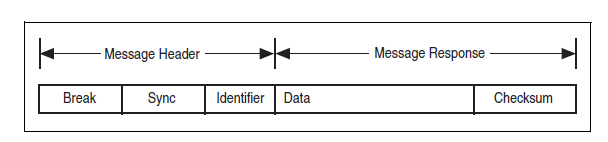
\includegraphics[width=0.4\textwidth]{LIN_frame.png}
  \caption{LIN frame}
  \label{fig:lin_frame}
\end{figure}

As shown in Figure~\ref{fig:lin_frame}, the LIN specification is very simple and
provides a small checksum for each message. Furthermore, to increase adoption of
LIN, the LIN standard provides an Application Programming Interface to design
LIN units against. This allows for software portability which further reduces
implementation costs. 

LIN is defined by it's simplicity, and low cost.  When performance is not
critical, and safety not paramount LIN is an excellent choice.  Stated another
way, when the designer wants something a bit more reliable than RS-232 without
resorting to a full safety critical protocol, LIN is
an excellent choice. 

\subsection{FlexRay}
FlexRay is a Class D, full duplex, network. It provides very high performance
at up to 10
Mbps while retaining a strong transmission error correction scheme.  FlexRay
supports both optical and electrical transport on the physical layer.  Optical
networks provide the strongest protection against EMI issues which further
contributes to FlexRay's reliability.  To
address availability, FlexRay divides transmission into major frames. Each major
frame is divided into two minor frames, a static frame and a dynamic frame. The
static frame implements a master schedule reserving fixed periods of
time called slots.  Each ECU on the network is assigned one or more slots for
that ECU to publish critical data. The dynamic phase allows for event triggered messages
similar to CAN \autocite{luo_research_2008}.  

\begin{figure}
  \centering
  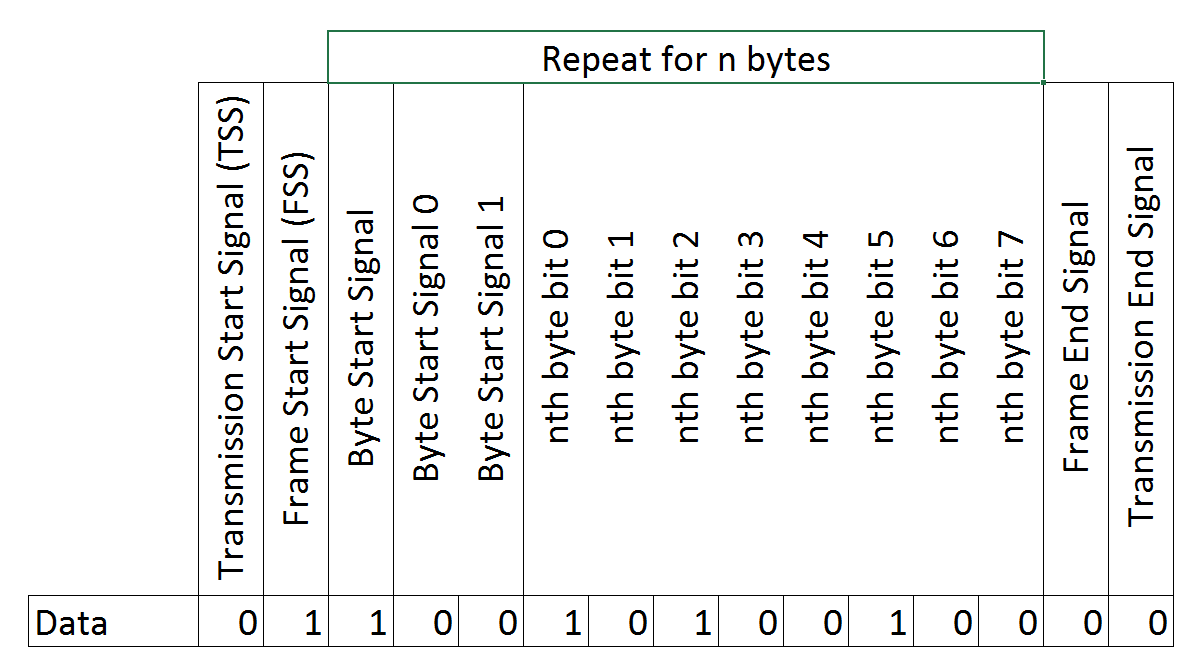
\includegraphics[width=0.4\textwidth]{Flexray.PNG}
  \caption{FlexRay frame}
  \label{fig:flexray_frame}
\end{figure}

For data integrity FlexRay provides a 24-bit CRC. FlexRay supports star
networks for highest performance, or multi-drop media for reduced cost. FlexRay
support dual channels each operating at up to 10 Mb/s. This adds extra
reliability. FlexRay pushes strict system requirements on maximum allowable clock
drift of 0.15\%. While this accuracy cannot be achieved with a standard
microcontroller RC oscillator, a quartz crystal oscillator can provide this
level of precision quite easily \autocite{_crystal_2014}. 

\section{FlexRay vs CAN}
Interestingly, FlexRay has been replacing CAN for many safety critical
systems. Systems such as BMW, and Mercedes' X-by-wire systems. FlexRay is also
being used in Mercedes' forward facing radar due to it high bandwidth, and high
reliability \autocite{guo_secure_2009}.  This comes from a side effect of CAN's
reliance on priority messaging.  Since CAN will always send the highest
priority message, most message schemes are designed on event based messaging.
The result, message that are important, but simply not \emph{most} important can
be delayed arbitrarily long on a busy CAN network. 

Cheng-lin shows how
FlexRay's reliability is independent of bus loading where CAN's reliability
degrades as the bus becomes loaded \autocite{cheng-lin_real-time_2010}.  In CAN
lower priority messages are held off while higher priority messages are
transfered summarized in Figure~\ref{fig:can_vs_flexray_reliability}. Cheng used
a Poisson error model, to describe how errors will propagate through a network,
and describe the probability of a message getting onto the bus. 

Cheng models the delay of low priority messages as
a function of the bus load. Intuitively, this makes sense, CAN messages are event
triggered, and both the software layers, and hardware layers route highest
priority messages first. Then if an important, but not quite the highest
priority
message is sitting in an ECU queue, it can wait a long period of time until it
has an opportunity to send the message.

Figure~\ref{fig:can_vs_flexray_reliability} shows that this error
exponentially approaches 100\% probability of failure. Eventually the bus fails
completely at a 
bus load of about 90\%. FlexRay however remains constant within this error
model using two mechanisms. Firstly, the static frame routes all priority messages according
to the defined schedule. This is the benefit of Time triggered networks,
something that \emph{could} be done with CAN, but wasn't part of the original
design. Secondly, FlexRay provides redundancy in two methods. Firstly FlexRay
defines a dual channel redundancy allowing a failed bus to send data over a back
channel. For the highest level of reliability however, FlexRay supports Dual
message, Dual channel which sends duplicate data over the redundant channel,
hence sending all messages twice.  This is the highest level of reliability and
according to Cheng results in a total probability of failure of $7.374 \times
10^{-50}$.

\begin{figure}
  \centering
  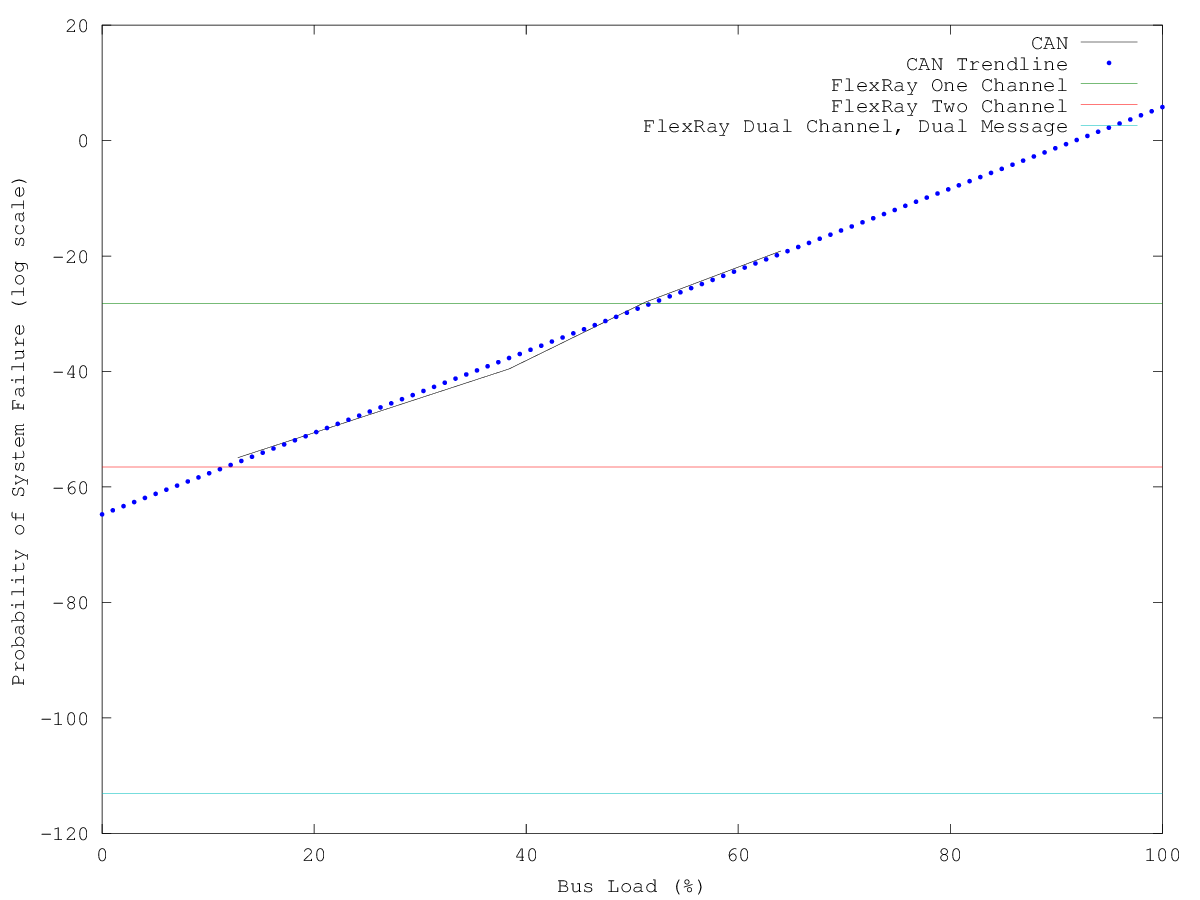
\includegraphics[width=0.4\textwidth]{FlexRaySystemReliability.png}
  \caption{CAN vs FlexRay Reliability}
  \label{fig:can_vs_flexray_reliability}
\end{figure}


\section{Messaging Schemes}
We've seen how the physical layer of CAN provides a priority scheme, but its
reliability is still susceptible to bus load factors. FlexRay's physical layer
however incorporates a two frame configuration to support both priority and time
based messages. Additionally, flexray provides dual channel and redundant messaging
resulting in a strongly reliable protocol.  However by stepping up a layer from
the physical, we can improve the reliability of CAN by incorporating some of
FlexRay's time trigger concepts \autocite{steinbach_tomorrows_2012}. 

This is the principle between message schemes.
At a layer above the physical layer, we can provide additional guarantees to
provide a more reliable channel. Similar to how TCP provides an in-order
guaranteed deliver over IP, we can provide guaranteed access for CAN.


\subsection{Time Triggered Messages}
\label{sec:time_trigger}
Time triggered message schemes send data at a rated defined by a network
``master schedule''. This is essentially time division multiplexing the
communication channel. The upside to time triggered messaging is the simplicity
of analysis. When all messages are defined for bounded windows of transmission,
all message latencies are explicitly know.  

The downside is
composability. Vehicle manufactures tend to build vehicle systems over time,
making small improvements and composing new functions reusing smaller functions
which already exist \autocite{ludanek_improved_2006}. Since the ``master
schedule'', is truly a single document describing all traffic, adding a new ECU
to the network requires the entire schedule to be redesigned and evaluated. One
method to deal with this is to design schedules with slack, or quiet periods.
Leaving room for future ECUs to fill the quiet time. This however isn't
scalable, requires a rgeat deal of time, and depending on what function comes in
the future may not even result in enough quiet time. Besides providing
guarenteed access even in high bus load situations Time triggered functions
provide another mechanism, fail safe. 

Time triggered messaging is primarily used in fail-safe systems such as steering
and braking. BMW's steer-by-wire systems use FlexRay for very high speed
communication, between the steering wheel, and the steering actuators. The
steering wheel periodically sends it's current angle, and velocity to the
actuator. If the actuator doesn't receive a message from the steering wheel on
the scheduled time, it can register a diagnostic trouble code to protect the vehicle
from a potentially failed steering wheel.  Braking is a similar design allowing
the vehicle to fail safely if communication channels are faulty
\autocite{wang_high_2011}. 

\subsection{Event Triggered Messages}
Event triggered schemes preserve bandwidth over time triggered schemes since
ECUs are not sending repeat messages. NMEA 0183 however combines these two
mechanisms. For reporting GPS position, NMEA 0183 defines two messages, a low speed
reference message called a COG sent at 1 Hz and high speed delta message called a SOG
\autocite{_nmea}. The
low speed message uses several CAN frames to publish a high accuracy gnss
position. The high speed message is sent at 10 Hz, and uses a single can frame.
This allows a time triggered scheme, but spreads the high precision updates over
time to preserve band width on the limited CAN bus.  By combining time trigger
and high speed update messages lower speed
buses such as Low speed CAN (125Kbps) more efficiently use the
limited performance. This however can make the latency more difficult to reason
about. If the message scheme doesn't support priority, as in LIN, and the ECU
doesn't internally route higher priority messages to the top when the master
initiates a transfer, then its possible for
lower priority messages to flood the bus, and prevent higher priority messages
from reaching the destination before the deadline. 

\section{System Architecture}
Now with various message schemes, over various transport, how are these pulled
together to a consistent system architecture.
Figure~\ref{fig:heterogenous_network} shows a typical breakdown of networks
according to the various functions within a vehicle. Initially, requirements are
broken down into the primary categories of vehicle networks.  Infotainment
systems include connectivity, GPS, music, and entertainment systems. These
systems are bandwidth heavy, but do not require high safety, for these MOST
(Media Oriented Service Transport) is typically used providing up to 12.5 Mbps.
Next comes the dash, and instrument panels. Typically these don't require high
bandwidth, but reliability and safety is paramount, this is a fit for time
triggered CAN.  Next comes electronic door locks, mirror adjustments, and other
simple control mechanisms. For these LIN is a great fit, since they require low
safety, and low speed.  Lastly, Engine, and transmission data. Drive by wire,
and electronic shifting. 
\begin{figure}
  \centering
  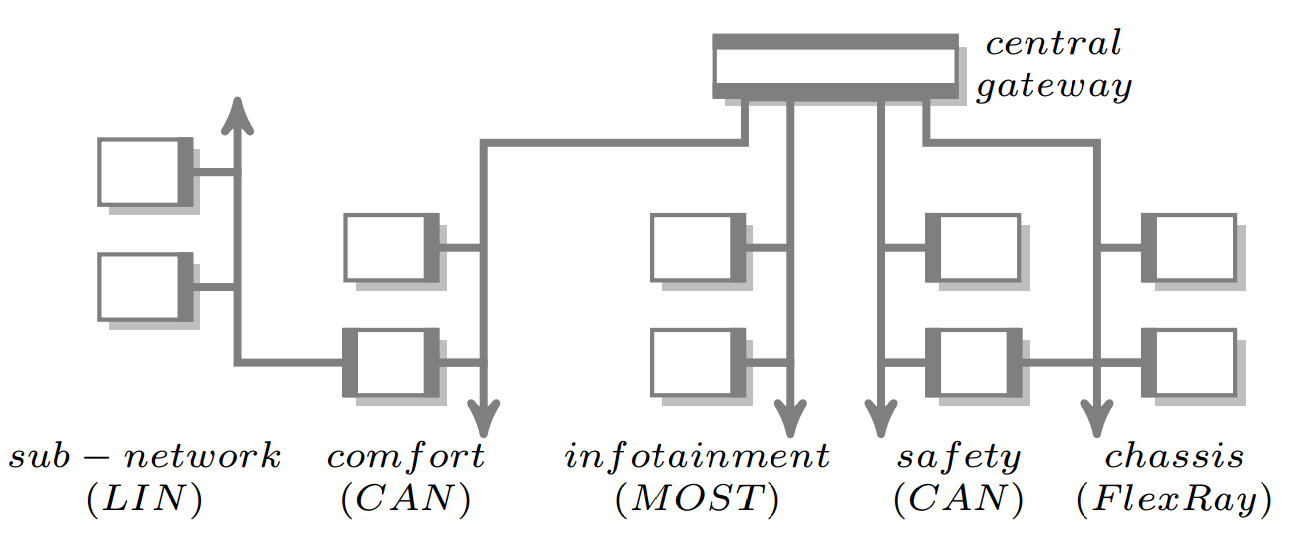
\includegraphics[width=0.4\textwidth]{network_topography.png}
  \caption{Heterogeneous Vehicle Network \autocite{lukasiewycz_system_2013}}
  \label{fig:heterogenous_network}
\end{figure}

Engines have grown exponentially in the amount of data they require to operate
properly. 
\section{Conclusion}
Each of the network types we've looked at are single media, multiple access
networks.  All ECUs, share a single set of wires to communicate to each other.
Ethernet is also such a configuration. However Ethernet's start of transmission
scheme is in start contract to industrial protocols presented here. Ethernet has
a randomized backoff scheme which manifest a variable network latency scheme.
If a device is a very loud talker, it can push out all other communication
creating a classic denial of service. In a vehicle bus, denial of service, i.e.
the steering wheel cannot contact the power steering unit as in a steer-by-wire
system. Such an event renders the vehicle an uncontrollable missile. But where Ethernet has variable latency
due to its randomized start of transmission scheme, industrial protocols have
two major schemes time triggered, and event triggered messaging for dealing with denial of service, and define a fixed
latency. 

Vehicle electronic are trending toward higher connectivity, higher security, and
greater integration within the vehicle as well as new out of vehicle systems.
These trends are already pushing the performance limits of its backbone protocol
CAN, and while MOST provides a higher bandwidth link, it cannot complete with
the safety offered by FlexRay.

As our vehicles are increasingly connect

It is an exciting time to see what advanced will be
made in the realm of vehicle protocols to meet this growing bandwidth bottleneck,
but maintain the critical safety specifications which keeps us blissfully unaware
of the mountain of software that make our cars function. 

\printbibliography

\end{document}
